\part{Implementación}\label{part:implementacion}

\section{Hardware}

\section{Firmware del microcontrolador}

\section{Aplicación de PC}\label{sec:pc}
La aplicación de PC es un programa con interfaz gráfica que permite al usuario administrar el contenido y configuración del cartel de forma remota. En el marco del protocolo definido en el \ref{sec:protocolo}, la aplicación de PC es el cliente.

\subsubsection{Plataforma de desarrollo}
La aplicación está desarrollada en el \emph{framework} de desarrollo Qt. Qt es un conjunto muy amplio de librerías que permiten el desarrollo de aplicaciones gráficas que se pueden compilar para distintas plataformas (Windows, GNU/Linux, macOS o cualquier variante de Unix con X11). El lenguaje de programación que se utiliza es C++ con extensiones propias de Qt.

\subsubsection{Arquitectura basada en eventos}\label{sec:qt}
Qt permite desarrollar aplicaciones con una arquitectura basada en eventos. Sin embargo, la implementación de este sistema de eventos no está basada en los mecanismos más clásicos como el patrón Observer de la programación orientada a objetos ni el mecanismo de callbacks o punteros a funciones propios de la programación procedural, sino que hay métodos en los objetos que pueden ser denominados \emph{signals} o \emph{slots}.

Una clase puede tener opcionalmente uno o más métodos que sean \emph{signal} o \emph{slot}. La idea clave de estas sistema es que un objeto puede \enquote{emitir} una \emph{signal} que ejecuta el método \emph{slot} de otro objeto (o incluso posiblemente el mismo emisor) al cual se estableció previamente lo que se denomina \enquote{conexión}. Se ilustra este mecanismo en la figura \ref{fig:signals-slots}

\begin{figure}[!ht]
	\centering
	\includegraphics[height=8cm]{imagenes/signal-slots.png}
	\caption{Mecanismo de \emph{signal} y \emph{slot}.}
	\label{fig:signals-slots}
\end{figure}

En Qt, las clases que necesiten utilizar el sistema de eventos deben heredar de una clase provista por la librería llamada \code{QObject}. Esta clase provee distintas funcionalidades al resto de las clases definidas por Qt. Entre los objetos que heredan de QObject puede existir una relación de parentesco, en la cual un objeto $B$ puede tener como padre a otro objeto $A$. Esto, por ejemplo, sirve para liberar al programador del manejo de memoria: un objeto puede destruir a sus hijos antes de destruirse a sí mismo (por destrucción se entiende la liberación de todo recurso asociado al objeto, como memoria o archivos).

El mecanismo de \emph{signal} y \emph{slots} tiene como una de sus ventajas el hecho de que la ejecución de un \emph{slot} darse en otro hilo. Esto esta relacionado con la idea que promueve Qt de que un objeto puede \enquote{pertenecer} a un hilo de ejecución (encapsulado por la clase \code{QThread}), esto permite que no haya interferencia de datos causada por la concurrencia ya que no hay accesos explícitos a variables compartidas entre hilos sino que pueden enviar datos como argumentos a los \emph{slots}, de forma similar al paradigma de pasaje de mensajes en programación concurrentes.

Por ejemplo, en el caso del objeto \code{Object1} en la figura \ref{fig:signals-slots}, en algún método suyo se podría tener código como el siguiente:
\begin{lstlisting}[language=c++]
	// ...
	emit signal1();
	// ...
\end{lstlisting}

Mientras que \code{Object2} tiene un \emph{slot} llamado \code{slot1()} al cual \code{signal1()} de \code{Object1} está conectado. Entonces al emitirse \code{signal1()}, se ejecuta también \code{slot1} de \code{Object2} (además de los otros métodos pertenecientes a las otras clases que aparecen en la figura).

El momento en que se ejecuta un \emph{slot} depende del tipo de conexión que se haya establecido entre los objetos. Qt define tres tipos de conexiones:
\begin{description}
	\item[\code{DirectConnection}:] el \emph{slot} se ejecuta en el mismo hilo de ejecución desde el cual se hizo la emisión. Esto es útil para cuando los objetos que están conectados pertenecen a un mismo hilo o también cuando pertenecen a distintos hilos pero se toma precaución utilizando primitivas de sincronización para serializar el acceso al recurso o memoria compartida.
	\item[\code{QueuedConnection}:] se coloca un pedido de ejecución de \emph{slot} (con los argumentos que se hayan emitido) en la cola de eventos del hilo del objeto destino. Esto es lo que libera al programador de tener que utilizar primitivas de sincronización explícitas y es lo que se usa mayormente en la aplicación de PC de este proyecto. La ejecución de \code{emit} retorna inmediatamente, con lo que el hilo del objeto emisor no se bloquea al emitir una señal.
	\item[\code{BlockingQueuedConnection}:] Similar a \code{QueuedConnection}, con la diferencia que el hilo emisor se bloquea hasta que finalice la ejecución de los \emph{slots} que haya activado. Si no se utiliza con precaución y se establecen conexiones cíclicas, existe el riesgo de que ocurra un \emph{deadlock}, ocurrencia en la que un conjunto de hilos se espera entre sí indefinidamente, deteniendo parcial o íntegramente el programa.
\end{description}

Internamente, la implementación de Qt tiene una cola bloqueante de eventos para cada uno de los hilos que tengan una instancia de la clase \code{QThread}. También lleva registro de cuáles objetos que heredan de \code{QObject} pertenecen a cuál hilo. De esta manera, la ejecución de un hilo consiste principalmente en esperar a que hayan eventos para procesar en una cola bloqueante, cuya implementación específica depende de la plataforma para la cual se esté compilando el programa.

\subsubsection{Módulos}
En esta sección se listan las clases más relevantes de la aplicación de PC, sus métodos públicos principales y la interacción entre ellos.
Las clases son:
\begin{description}
	\item[\code{Panel}:] Provee la interfaz gráfica principal, que consiste en una ventana con los distintos elementos de control para que el usuario pueda manipular el cartel. Se puede ver una captura de pantalla en la figura \ref{fig:panel-screenshot}.
	\item[\code{Client}:] Realiza la interacción con el cartel a nivel mensaje del protocolo. Se encarga de generar los mensajes salientes y de tomar las acciones pertinentes ante una respuesta del cartel (servidor). La (única) instancia de esta clase \enquote{pertenece} (ver sección \ref{sec:qt}) a otro hilo en el cual se realizan todas las operaciones bloqueantes de entrada y salida, de forma que no se bloquea el hilo principal, que causaría que la interfaz gráfica deje de responder a eventos del sistema o del usuario.
	\item[\code{Connection}:] Abstrae la conexión al cartel, exponiendo métodos que envían y reciben específicamente los mensajes definidos en el protocolo. En esta clase también se hace la carga del certificado TLS antes de establecer una conexión.
	\item[\code{SignModel}:] Una clase \enquote{tonta} que agrupa todos los parámetros modificables del cartel, como el texto del cartel y sus parámetros de animación, los datos de la red Wifi a la que se debe conectar el cartel, etc. Existe principalmente para llevar registro de cuales parámetros fueron cambiados por el usuario y ameritan un pedido de cambio hacia el cartel. De manera que no se hagan cambios innecesarios al contenido o configuración del cartel.
\end{description}

Se puede ver en la figura \ref{fig:uml-cliente} un diagrama de los objetos mencionados anteriormente. No están incluidas las conexiones entre los objetos para mantener la prolijidad del diagrama.

Los objetos están repartidos entre los dos hilos como se muestra en la figura \ref{fig:qt-threads}.

\begin{figure}[!ht]
	\centering
	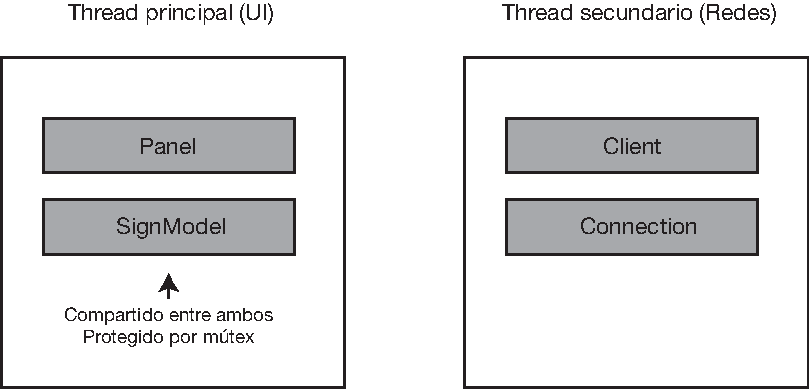
\includegraphics[scale=0.8]{imagenes/qt-threads.pdf}
	\caption{Distribución de los objetos en hilos.}
	\label{fig:qt-threads}
\end{figure}

\begin{figure}[!ht]
	\centering
	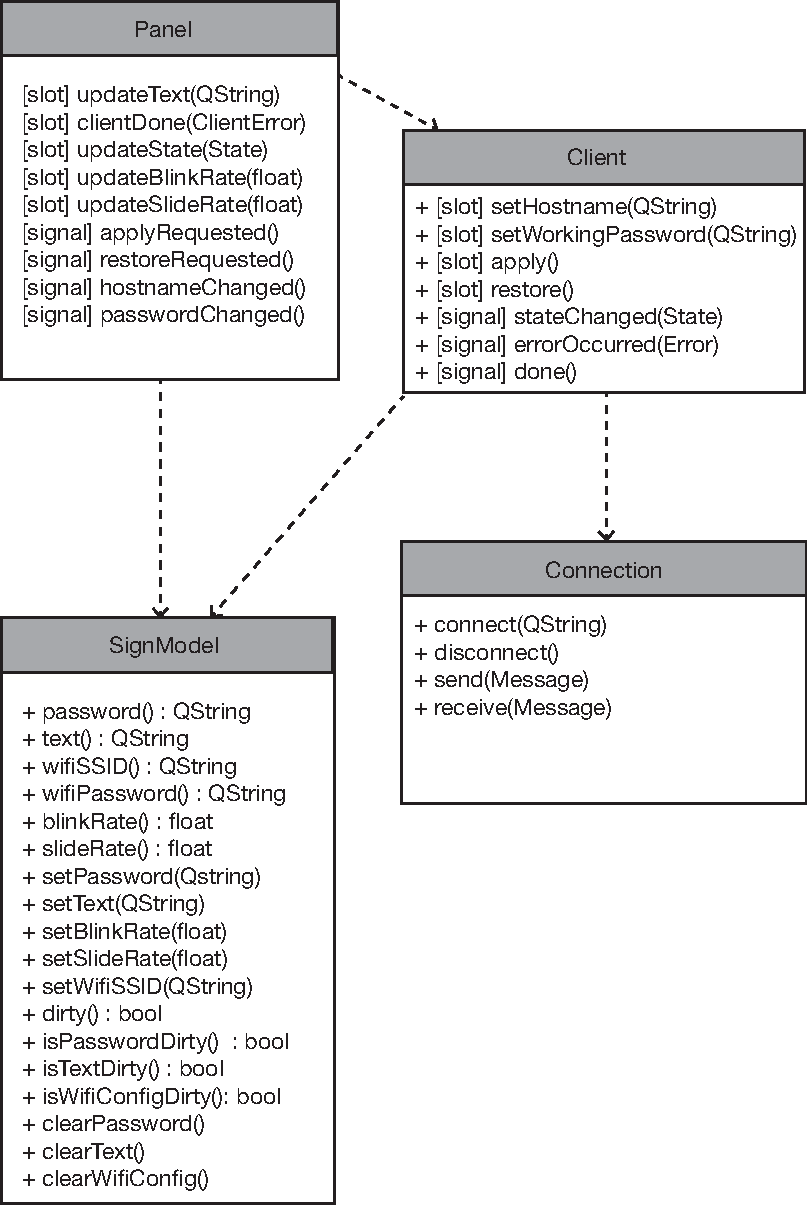
\includegraphics[scale=0.8]{imagenes/uml-cliente.pdf}
	\caption{Diagrama UML de las clases más relevantes.}
	\label{fig:uml-cliente}
\end{figure}

\begin{figure}[!ht]
	\centering
	\includegraphics[height=10cm]{imagenes/panel-screenshot.png}
	\caption{Captura de pantalla de la ventana principal de la aplicación de pc.}
	\label{fig:panel-screenshot}
\end{figure}

\paragraph{Panel}
La clase Panel implementa la interfaz gráfica mediante la cual el usuario ingresa y visualiza el contenido y configuración del cartel. Sus métodos no deben hacer operaciones que tarden, ya que eso resultaría en que la interfaz de usuario se congele. Por esto y para lograr una mejor separación de propósito en las clases, la clase Panel solo se encarga de este aspecto del programa.

Un flujo típico de ejecución es el siguiente:
\begin{enumerate}
	\item La clase se inicializa a su misma y sus objetos asociados (entre ellos, una instancia de Client y una de SignModel).
	\item Se muestra el diálogo en el cual se ingresa la dirección de IP o nombre de host del cartel a cual conectarse. Ver figura \ref{fig:login}
	\item Asumiendo que no se seleccionó \enquote{Cancelar} en el diálogo anterior, el objeto Panel inicia una interacción para traer el estado (contenido y configuración) del cartel. Hace esto emitiendo la señal \code{restoreRequested()}, que está conectada al \emph{slot} \code{apply()} del objeto de clase Client.
	\item El objeto de tipo Panel desactiva todos los elementos de la interfaz gráfica de forma que no se pueda realizar otra operación mientras haya una interacción en curso.
	\item El objeto de tipo Panel continúa procesando los eventos de la cola de eventos normalmente. Uno de estos eventos será una señal \code{done(ClientError)} de Client, conectada al \emph{slot} \code{clientDone(ClientError)} de Panel. El argumento es un enumerativo que representa un error o éxito. También, durante el transcurso de una interacción, Client va emitiendo señales para notificar de cambios de su estado interno, para poder mostrar mensajes al usuario sobre la fase de la interacción actual (\enquote{Conectando},\enquote{Esperando respuesta...}, etc).
\end{enumerate}

\begin{figure}[hbtp]
	\centering
	\includegraphics[scale=0.8]{imagenes/login.png}
	\caption{Captura de pantalla de la ventana de login.}
	\label{fig:login}
\end{figure}

\paragraph{Client}
Client es la clase que implementa la interacción en si a nivel mensajes de protocolo. Es decir, es la clase que sabe qué mensajes emitir y que hacer ante las respuestas.

Cuando se inicia una interacción del tipo \enquote{get}, simplemente inicia una conexión (utilizando un objeto de tipo Connection), y realiza dos interacciones en la misma conexión: una para traer el contenido del cartel y otra para traer la configuración de WiFi.

Por otro lado, cuando se inicia una interacción del tipo \enquote{set}, debe primero determinar cuales partes del módelo del cartel han cambiado y deben, por ende, ser actualizadas. Para eso usa unos métodos de SignModel que permiten cuales datos han sido cambiados por el usuario. Estos son: \code{isPasswordDirty()}, \code{isTextDirty()} y \code{isWifiConfigDirty()}.

A lo largo de una interacción, el objeto de tipo Client va cambiando de estados. Internamente tiene un enumerativo con los siguientes valores:
\begin{description}
	\item[Disconnected:] Client está listo para iniciar una interacción.
	\item[Connecting:] Se envió una solicitud de conexión y se está esperando una respuesta.
	\item[Connected:] Se recibió una respuesta a la solicitud de conexión y hay una conexión establecida.
	\item[RequestSent:] Se envió un pedido (ver sección \ref{sec:protocolo}) y se espera una respuesta.
	\item[ResponseReceived:] Se recibió una respuesta y se está procesándola.
\end{description}

Los estados Connected y ResponseReceived existen más bien por completitud, ya que el tiempo en que se permanece en esos estados no es perceptible.

También se define en esta clase un enumerativo \code{ClientError}, que representan los distintos errores en los que puede finalizar una interacción. Tiene los siguientes valores:
\begin{description}
	\item[Ok:] La interacción fue exitosa.
	\item[CertificateMissing:] No se pudo cargar el certificado TLS.
	\item[Timeout:] Se excedió el tiempo de espera a una respuesta.
	\item[WrongResponse:] Se recibió una respuesta incorrecta por parte del servidor. Esto puede suceder si hay un error en la implementación del protocolo, o si a lo que se conectó no es un cartel, sino algun otro servicio sobre TLS, como un servidor web con HTTPS.
	\item[IncompleteWrite:] No se pudo mandar un mensaje entero. Se debe a un problema externo de red.
	\item[ConnectionRefused:] El host remoto rechazó la conexión. Muy posiblemente no sea un cartel.
	\item[RemoteHostClosed:] El host remoto cerró inesperadamente la conexión. Esto puede pasar si alguna fase de la interacción tardo demasiado (por congestión de la red, por ejemplo), haciendo que el cartel cierre la conexión.
	\item[HostNotFound:] No se pudo resolver la dirección IP del nombre de host dado.
	\item[NetworkError:] Error de red genérico.
	\item[SslHandshakeFailed:] Falló el establecimiento de una conexión TLS. Esto puede darse por certificados y claves que no coinciden, corrupción de ellos o un error en la implementación de TLS del ESP8266EX.
	\item[SslInternalError:] Error interno de OpenSSL (librería que maneja las conexiones TLS).
	\item[SslInvalidData:] El certificado público cargado no es válido.
	\item[Unknown:] Error desconocido genérico.
	\item[ServerMalformedPacket:] Se recibió un paquete no conforme a lo descrito por la especificación del protocolo.
	\item[ServerBadPassword:] Se trató de iniciar una interacción con una contraseña incorrecta.
	\item[ServerBadProtocolVersion:] El cartel tiene una versión del protocolo más nueva que la de la aplicación de PC.
\end{description}
\paragraph{Connection}
Esta clase es más pequeña que las anteriores. Provee una interfaz simple para iniciar una conexión TLS y mandar mensajes. Tiene los siguientes métodos bloqueantes:
\begin{description}
	\item[\code{bool connect(const QString hostname)}:] Inicia una conexión TLS al host con nombre dado por \code{hostname}. Retorna falso si hubo error o timeout.
	\item[\code{bool disconnect()}:] Cierra la conexión. Es idempotente: si no existía previamente una conexión abierta, no realiza ninguna acción.
	\item[\code{bool send(const Message \&msg)}:] Envia el mensaje \code{msg}. Retorna falso si hay error o timeout.
	\item[\code{bool receive(Message \&msg)}:] Recibe un mensaje y lo almacena en \code{msg}. Retorna falso si hay error o timeout.
	\item[\code{QAbstractSocket::SocketError lastError()}:] Retorna un enumerativo con el último error de red. Este enumerativo es propio de Qt y luego se mapea a un valor del enumerativo \code{Client::ClientError}.
\end{description}

Todos estos métodos tienen un tiempo de expiración o \emph{timeout} definido por la constante estática \code{Connection::TIMEOUT\_MS}

